\documentclass[11pt,a4paper]{article}
\usepackage[margin=0.82in,headheight=15pt,headsep=18pt]{geometry}
\usepackage[T1]{fontenc}
\usepackage{mathptmx}
\usepackage[scaled=0.94]{helvet}
\usepackage{microtype,graphicx,tikz,pgfplots,booktabs,array,tabularx}
\usepackage{xcolor,caption,fancyhdr,titlesec,hyperref,enumitem,xurl,embedfile}
\usetikzlibrary{arrows.meta,positioning,calc}
\pgfplotsset{compat=1.18}
\definecolor{ink}{HTML}{192C3B}
\definecolor{accent}{HTML}{23685E}
\definecolor{muted}{HTML}{56636C}
\definecolor{chipgray}{HTML}{F0F1F2}
\definecolor{linegray}{HTML}{D8DEE1}
\hypersetup{colorlinks=true,linkcolor=accent,urlcolor=accent,pdftitle={Hypothesis-Tree Agents for Molecular Discovery},pdfauthor={}}
\setlength{\parindent}{0pt}
\setlength{\parskip}{7pt}
\linespread{1.07}
\titleformat{\section}{\Large\sffamily\bfseries\color{ink}}{\thesection.}{0.5em}{}
\titlespacing*{\section}{0pt}{14pt}{9pt}
\titleformat{\subsection}{\normalsize\sffamily\bfseries\color{accent}}{}{0pt}{}
\titlespacing*{\subsection}{0pt}{11pt}{3pt}
\captionsetup{hypcap=false,font=small,labelfont=bf,justification=raggedright,singlelinecheck=false,skip=7pt}
\pagestyle{fancy}\fancyhf{}
\fancyhead[L]{\footnotesize\sffamily\color{muted}HYPOTHESIS-TREE AGENTS}
\fancyhead[R]{\footnotesize\sffamily\color{muted}RESEARCH PROPOSAL}
\fancyfoot[L]{\footnotesize\sffamily\color{muted}October 2026}
\fancyfoot[R]{\footnotesize\sffamily\color{muted}\thepage}
\renewcommand{\headrulewidth}{0.3pt}
\newcommand{\chip}[1]{\tikz[baseline=(label.base)]\node[fill=chipgray,rounded corners=2pt,inner xsep=5pt,inner ysep=3pt,font=\normalfont\normalsize] (label) {\strut #1};}
\setlist[itemize]{leftmargin=1.2em,itemsep=5pt,topsep=4pt,parsep=0pt}
\newcommand{\level}[1]{\subsection*{#1}}
\tikzset{flow/.style={draw=linegray,fill=chipgray,rounded corners=4pt,align=left,inner sep=9pt,font=\small,text width=4.65cm,minimum height=1.3cm}, arrow/.style={-{Latex[length=2mm]},line width=.8pt,draw=accent}}
\begin{document}
\thispagestyle{fancy}
{\small\sffamily\bfseries\color{accent}AUTONOMOUS SCIENTIFIC DISCOVERY}\par\vspace{7pt}
{\fontsize{27}{30}\selectfont\sffamily\bfseries\color{ink}Hypothesis-Tree Agents\\for Molecular Discovery}\par
\vspace{4pt}
{\large\color{muted}Learning from experiments through persistent scientific memory}\par
\vspace{12pt}
\colorbox{chipgray}{\parbox{\dimexpr\linewidth-2\fboxsep\relax}{\vspace{6pt}\textbf{Proposal in brief.} Build a molecular research agent that turns each experiment into a reusable paper, selects its next question from a branching research history, and improves a hidden objective through evidence-guided experimentation.\vspace{6pt}}}

\section{Introduction}
Molecular discovery is a sequential learning problem: each candidate should teach us something useful about the next experiment. A black-box oracle makes this particularly demanding. The agent can submit a molecular structure and observe a scalar score, but cannot inspect the objective's formula or gradients. The central research question is whether an agent can make these evaluations more informative by maintaining an explicit record of what it tried, what improved, what failed, and which explanations remain uncertain.

We propose a \textbf{hypothesis tree} as the agent's scientific memory. Each node represents a testable hypothesis and its completed experiment, documented as a short research paper. A child builds on a committed parent; siblings test distinct claims arising from the same research state. This organization lets the agent deepen a promising lineage, revisit an earlier question, or compare evidence across branches without discarding negative results. The tree therefore stores both successful molecules and the reasoning needed to design subsequent tests.

A Qwen language model operates through a ReAct loop: it reasons about the current evidence, chooses a structured action, observes the result, and revises its next step. Persistent notes support work in progress; published papers preserve the verified experimental record. The intended contribution is an agent that improves its \emph{experimental decisions} as evidence accumulates, without requiring model-weight updates during a campaign.

\begin{center}
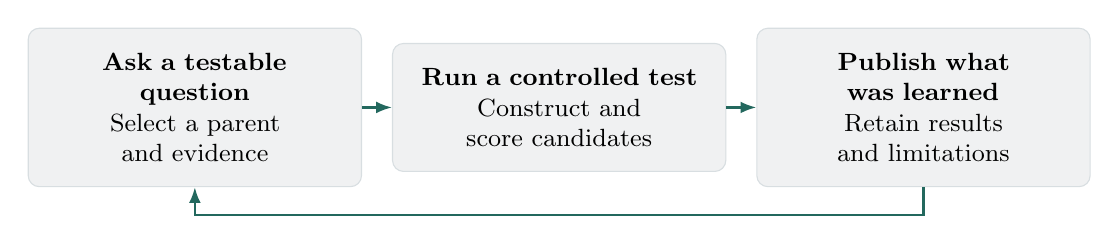
\begin{tikzpicture}[font=\small,every node/.style={align=center}]
\node[flow,text width=3.6cm,align=center] (q) {\textbf{Ask a testable question}\\Select a parent and evidence};
\node[flow,text width=3.6cm,align=center,right=0.38cm of q] (e) {\textbf{Run a controlled test}\\Construct and score candidates};
\node[flow,text width=3.6cm,align=center,right=0.38cm of e] (p) {\textbf{Publish what was learned}\\Retain results and limitations};
\draw[arrow] (q)--(e);\draw[arrow](e)--(p);
\draw[arrow] (p.south)--++(0,-.35)-|(q.south);
\end{tikzpicture}
\end{center}
The campaign examined here improved the measured score from \textbf{0.368 to 0.905}, with \textbf{83 unique scored molecules including initialization} and \textbf{48 completed experiment papers}. These results motivate a broader evaluation of whether structured scientific memory improves discovery efficiency and the quality of the hypotheses an agent chooses.

\newpage
\section{Action space}
The action interface makes scientific work explicit. Each turn returns a structured envelope, \textsf{\{reason, action, args\}}, containing a concise rationale and one action. The available actions depend on the current phase, while reads and notes can recur as often as needed within that phase.

\renewcommand{\arraystretch}{1.2}
\begin{tabularx}{\linewidth}{@{}p{0.40\linewidth}X@{}}
\toprule
\textbf{Action} & \textbf{Scientific purpose}\\
\midrule
\chip{inspect\_tree} & View paginated node summaries and locate promising or unresolved research lines.\\[7pt]
\chip{read}\quad\chip{search}\quad\chip{compare} & Retrieve paper sections, find relevant prior experiments, and compare measured outcomes across nodes.\\[7pt]
\chip{deep\_read} & Ask a dedicated reader to extract evidence, limitations, and candidate hypotheses into a saved note.\\[7pt]
\chip{write\_note} & Record working hypotheses, observations, and source references in the current workspace.\\[7pt]
\chip{select\_parent} & Choose a committed experiment and a measured reference molecule for the next research question.\\[7pt]
\chip{propose\_hypotheses} & Formulate two distinct child claims with predictions and outcomes that would challenge them.\\[7pt]
\chip{submit\_matrix} & Freeze explicit candidate structures in a bases-by-strategies experiment matrix for oracle evaluation.\\[7pt]
\chip{submit\_observation} & Interpret the receipts; distinguish hypothesis support from an improvement in score.\\[7pt]
\chip{submit\_paper} & Publish the hypothesis, methods, results, limitations, and conclusions as an immutable experiment record.\\
\bottomrule
\end{tabularx}

\vspace{7pt}
\textbf{From retrieval to reusable memory.} Reading and searching are purposeful experimental actions: a negative result may rule out an attractive edit, while a comparison may reveal that two competing explanations make different predictions. Notes retain those distinctions before the agent commits to a new test. Context continuation preserves unfinished work when a model session fills.

\begin{center}
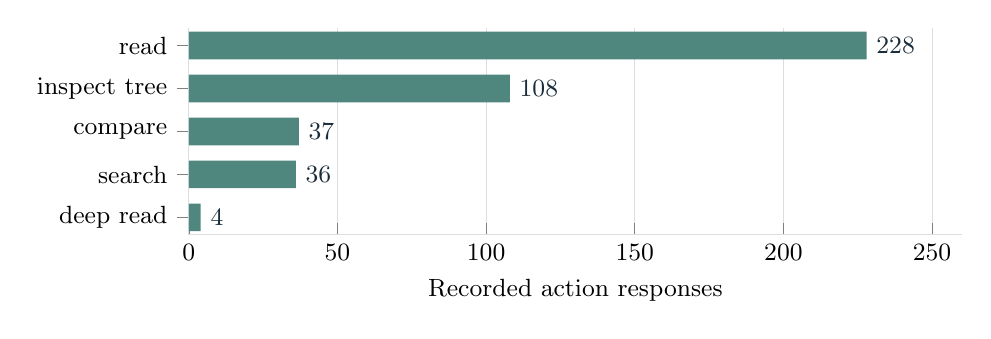
\begin{tikzpicture}
\begin{axis}[xbar,width=.94\linewidth,height=4.2cm,xmin=0,xmax=260,
 symbolic y coords={deep read,search,compare,inspect tree,read},ytick=data,
 tick label style={font=\small},xlabel={Recorded action responses},xlabel style={font=\small},
 axis x line*=bottom,axis y line*=left,axis line style={draw=linegray},
 xtick={0,50,100,150,200,250},xmajorgrids=true,grid style={linegray},
 nodes near coords,nodes near coords style={font=\small,text=ink},bar width=10pt]
\addplot[fill=accent!80,draw=none] coordinates {(4,deep read)(36,search)(37,compare)(108,inspect tree)(228,read)};
\end{axis}
\end{tikzpicture}
\captionof{figure}{Selected memory actions from the campaign. Frequent reads and tree inspections motivate testing whether more targeted retrieval can preserve discovery quality with less overhead.}
\end{center}

\newpage
\section{How this works}
At time $t$, the agent receives a bounded view of the current research tree, the task brief, and the available evidence references. It inspects the tree and selects a committed parent with a scored molecule as its comparison point. Parent selection determines the question's experimental lineage; it does not erase other branches or reset the campaign's best observed score.

\begin{center}
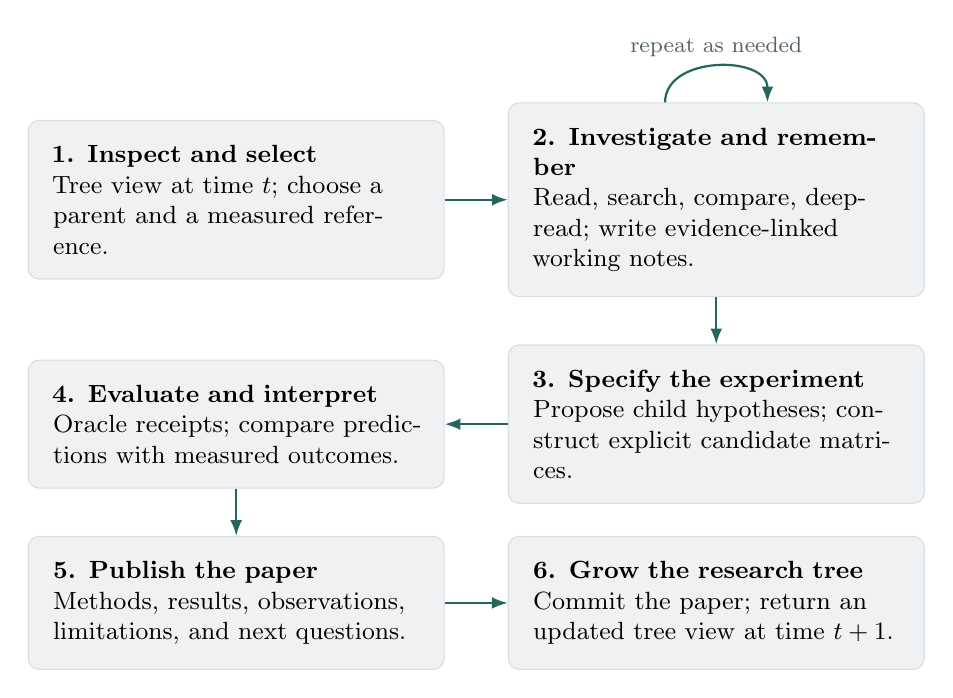
\begin{tikzpicture}
\node[flow] (a) {\textbf{1. Inspect and select}\\Tree view at time $t$; choose a parent and a measured reference.};
\node[flow,right=.8cm of a] (b) {\textbf{2. Investigate and remember}\\Read, search, compare, deep-read; write evidence-linked working notes.};
\node[flow,below=.6cm of b] (c) {\textbf{3. Specify the experiment}\\Propose child hypotheses; construct explicit candidate matrices.};
\node[flow,left=.8cm of c] (d) {\textbf{4. Evaluate and interpret}\\Oracle receipts; compare predictions with measured outcomes.};
\node[flow,below=.6cm of d] (e) {\textbf{5. Publish the paper}\\Methods, results, observations, limitations, and next questions.};
\node[flow,right=.8cm of e] (f) {\textbf{6. Grow the research tree}\\Commit the paper; return an updated tree view at time $t+1$.};
\draw[arrow](a)--(b);\draw[arrow](b)--(c);\draw[arrow](c)--(d);\draw[arrow](d)--(e);\draw[arrow](e)--(f);
\draw[arrow] ([xshift=-.65cm]b.north) .. controls +(0,.6cm) and +(0,.6cm) .. node[above,font=\footnotesize,text=muted]{repeat as needed} ([xshift=.65cm]b.north);
\end{tikzpicture}
\captionof{figure}{One research cycle. ReAct governs repeated decisions within the permitted phase; the experimental record persists across cycles.}
\end{center}

\textbf{Reasoning with working memory.} ReAct is the decision loop throughout the investigation. The agent can inspect a paper, observe a failed substitution, search for a related comparison, and write a note explaining how that result changes its next hypothesis. A dedicated reader can add a focused synthesis. These notes belong to the active workspace and can be cited or inherited by the subsequent hypothesis experiments.

\textbf{Turning a hypothesis into a test.} The agent states a claim, its rationale, a prediction, and an outcome that would challenge it. It then specifies a small matrix of starting structures and concrete interventions. Each cell contains the actual candidate molecule to be evaluated; the backend does not invent molecular edits. Freezing the matrix makes the intended experiment distinguishable from its subsequent interpretation.

\textbf{Closing the loop with evidence.} The backend validates and canonicalizes candidates, reuses cached scores for duplicates, and records new oracle evaluations. Invalid structures remain visible as construction failures. The observer compares the returned receipts with the prediction, then the reporter writes the full experiment paper. A Git-backed commit preserves the paper and verified matrix as a new tree node. Future decisions can retrieve its positive, negative, or inconclusive findings rather than relying on an ephemeral conversation.

\newpage
\section{An agent's trajectory}
This session began with an unnamed structure and progressed through increasingly focused experiments. Tree levels denoted experimental ancestry; the agent learned through recorded evidence rather than model-weight updates.

\level{Level 0: established the starting point}
\begin{itemize}
\item The agent received a black-box task brief and one structure scoring \textbf{0.368}. It was not given the objective identity or formula.
\item It recorded the baseline and proposed structural changes that could reveal which parts of the molecule mattered.
\end{itemize}

\level{Level 1: found a productive direction}
\begin{itemize}
\item The agent tested aryl substitutions, but both candidates fell to \textbf{0.305}. Simple terminal-amine $N$-methylation also underperformed at \textbf{0.339}.
\item A piperazinyl side chain raised the score to \textbf{0.857}. The agent pursued that branch while keeping the cause of the gain unresolved.
\end{itemize}

\level{Level 2: narrowed the hypothesis}
\begin{itemize}
\item The agent compared distal $N$-alkylation (best \textbf{0.849}), halogen swaps (\textbf{0.797}), and ring-identity changes (\textbf{0.857}). Ester and linker edits also failed to improve the reference.
\item Ring size proved more useful: seven members scored \textbf{0.844}, while five reached \textbf{0.871}. That contrast motivated a test of further ring contraction.
\end{itemize}

\begin{center}
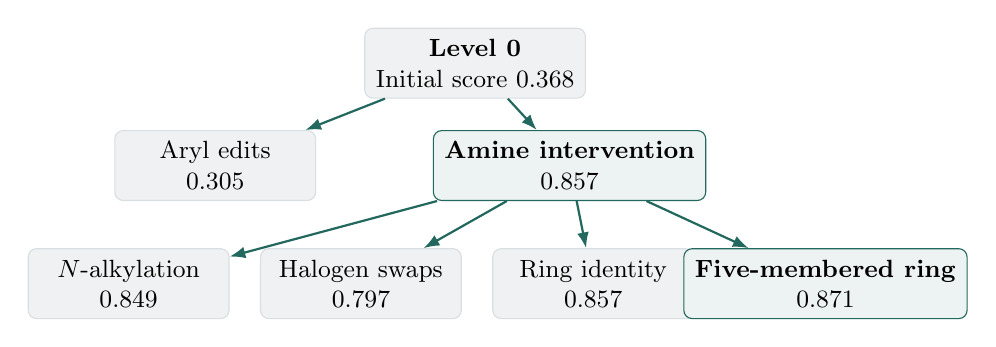
\begin{tikzpicture}[font=\small, every node/.style={align=center},
 n/.style={draw=linegray,fill=chipgray,rounded corners=3pt,minimum width=2.55cm,minimum height=.77cm,inner sep=4pt},
 w/.style={n,draw=accent,fill=accent!8},e/.style={arrow}]
\node[n] (r) at (0,0) {\textbf{Level 0}\\Initial score 0.368};
\node[n] (a) at (-3.3,-1.3) {Aryl edits\\0.305};
\node[w] (b) at (1.2,-1.3) {\textbf{Amine intervention}\\0.857};
\node[n] (c) at (-4.4,-2.8) {$N$-alkylation\\0.849};
\node[n] (d) at (-1.45,-2.8) {Halogen swaps\\0.797};
\node[n] (e) at (1.5,-2.8) {Ring identity\\0.857};
\node[w] (f) at (4.45,-2.8) {\textbf{Five-membered ring}\\0.871};
\draw[e](r)--(a);\draw[e](r)--(b);
\draw[e](b)--(c);\draw[e](b)--(d);\draw[e](b)--(e);\draw[e](b)--(f);
\end{tikzpicture}
\captionof{figure}{Selected early experiments. Green outlines identify improvements along the lineage continued below. Each child is an experiment; labels report its best candidate score.}
\end{center}

\newpage
{\large\sffamily\bfseries\color{ink}Agent trajectory, continued}\par
\level{Levels 3 and 4: extended the successful trend}
\begin{itemize}
\item At level 3, the agent tested a four-membered terminal ring and reached \textbf{0.889}. Core-methyl edits and a methyl-substituted five-membered ring did worse, strengthening the case for ring contraction.
\item At level 4, it tested a three-membered diaza ring against the four-membered reference and reached \textbf{0.905}, the session's best observed score. A separate nitrogen-position isomer tied its parent and added no improvement.
\end{itemize}

\begin{center}
\begin{tabular}{@{}c@{\hspace{.6cm}}c@{}}
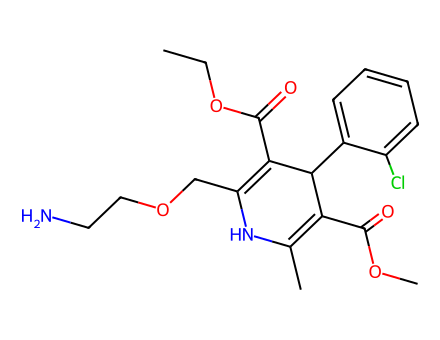
\includegraphics[width=.43\linewidth,height=3.5cm,keepaspectratio]{figs/l0.png} &
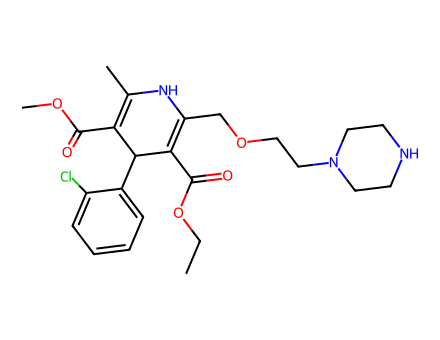
\includegraphics[width=.43\linewidth,height=3.5cm,keepaspectratio]{figs/l1.png}\\[-2pt]
{\small\textbf{Level 0} $\cdot$ 0.368} & {\small\textbf{Level 1} $\cdot$ 0.857}\\[6pt]
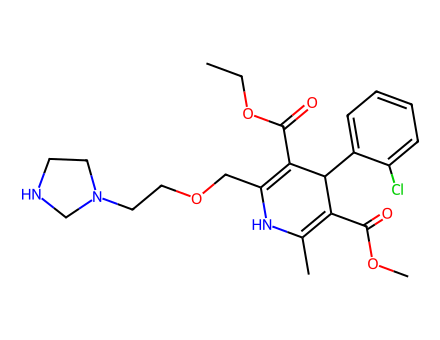
\includegraphics[width=.43\linewidth,height=3.5cm,keepaspectratio]{figs/l2.png} &
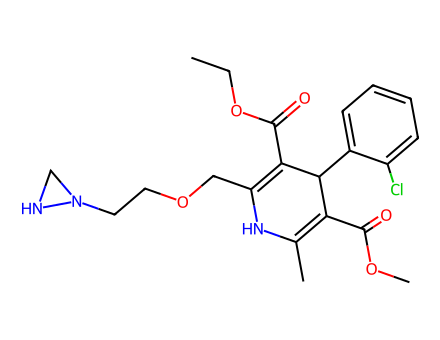
\includegraphics[width=.43\linewidth,height=3.5cm,keepaspectratio]{figs/best.png}\\[-2pt]
{\small\textbf{Level 2} $\cdot$ 0.871} & {\small\textbf{Level 4} $\cdot$ 0.905}
\end{tabular}
\captionof{figure}{Selected structures along the improving lineage: initial molecule, level-1 cyclic-amine candidate, level-2 five-membered ring, and level-4 three-membered ring. Scores rise from 0.368 to 0.857, 0.871, and 0.905; the intermediate level-3 result is 0.889.}
\end{center}

\level{Levels 5 and 6: revised the explanation and tested the limits}
\begin{itemize}
\item The agent found that removing one or both terminal-ring nitrogens preserved \textbf{0.905}. This challenged its earlier explanation that the two-nitrogen pattern was essential.
\item Ring enlargement, linker changes, core $N$-alkylation, and further aryl edits did not exceed the incumbent. The session ended with a stronger candidate and a clearer record of useful and unsuccessful interventions, without establishing a global optimum.
\end{itemize}

\newpage
\section{Research agenda and expected contribution}
\subsection*{Two directions for improving the agent}
\textbf{Learn a more selective tool policy.} The action profile shows substantial reading and tree-inspection activity. Supervised fine-tuning or reinforcement learning could encourage targeted retrieval, useful note writing, and informative comparisons. The objective should balance discovery quality with model and oracle cost; a lower number of reads is valuable only if the agent retains the evidence needed for good experimental decisions.

\textbf{Improve search across the research tree.} Better parent selection could combine promising scores with unresolved scientific questions, evidence coverage, and the expected value of a comparison. Longer deliberation may be useful when several papers support incompatible explanations. Adaptive experiment allocation should be evaluated against the frozen-matrix prototype, with the same accounting for calls, duplicates, and construction failures.

\subsection*{Expected contribution}
The intended result is a reusable architecture coupling molecular search with persistent experimental memory. Success would show that accumulated evidence improves experiment selection and discovery efficiency, with every gain traceable to a candidate, an oracle receipt, and an evidence-grounded paper.


\newpage
\appendix
\section{Inspecting an experiment node}
\begin{minipage}[c]{.48\linewidth}
\centering
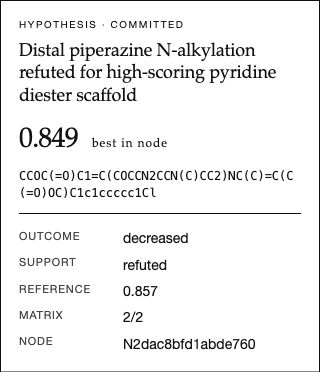
\includegraphics[width=7cm]{figs/node-hover-card.jpg}
\end{minipage}\hfill
\begin{minipage}[c]{.48\linewidth}
This actual hover card summarized a level-2 experiment in the session. It showed the best measured molecule, score, parent reference, matrix completion, and separate assessments of objective outcome and hypothesis support.

Here, distal $N$-alkylation scored below its parent: \textbf{0.849 versus 0.857}. The card marked the hypothesis as refuted. Opening the node led to the full experiment paper, reproduced in Appendix~\ref{app:paper}.
\end{minipage}
\begin{minipage}{\linewidth}\captionof{figure}{Screenshot of the campaign interface for node N2dac8bfd1abde760. The same node's committed paper appears in the appendix.}\end{minipage}

\vfill
{\footnotesize\color{muted}\textbf{Evidence basis.} Campaign-v2 ledger and committed experiment papers. The 83 unique scored molecules comprise initialization and 82 newly scored matrix cells; cached and invalid cells are excluded. Forty-eight experiment papers were completed. Research directions above are future work.}

\newpage
\section{An actual agent-produced paper}\label{app:paper}
This paper was retrieved from the immutable Git record of the node shown in Appendix~A. Its narrative was reproduced verbatim with typesetting changes; the verified results were reformatted. The complete original Markdown, including frozen hypotheses, plan, observations, and receipts, was embedded as a PDF attachment.

{\small\color{muted}\textbf{Source node:} N2dac8bfd1abde760\\
\textbf{Git commit:} \nolinkurl{93ee8f368ad703a59f49d501f8b2745918971f61}}
\embedfile[desc={Original agent-produced experiment paper, including all backend records},mimetype={text/markdown}]{actual-node-paper.md}
\begingroup
\fontsize{10.5}{12}\selectfont
\urlstyle{same}
\setlength{\parskip}{4pt}
\titlespacing*{\subsection}{0pt}{6pt}{2pt}
\subsection*{Distal piperazine N-alkylation refuted for high-scoring pyridine diester scaffold}

{\small\setlength{\parskip}{0pt}
{Node: \nolinkurl{N2dac8bfd1abde760}\par}
{Research parent: \nolinkurl{N0c05b43f5289a00a}\par}
{Expansion: \nolinkurl{Xa8bbe7f04df1b3e3} (sibling 0)\par}
{Hypothesis support (Qwen assessment): refuted\par}
{Objective outcome (backend): decreased\par}
{Parent reference: \nolinkurl{Cec74c6f32634804f} \nolinkurl{CCOC(=O)C1=C(COCCN2CCNCC2)NC(C)=C(C(=O)OC)C1c1ccccc1Cl} score 0.857143\par}
{Plan hash: \nolinkurl{e7c6731a7f11460f55b2f4f0884065c24fe24ae666cb8a421386028055ad498e}\par}

}
\subsection*{Search gist}
We tested whether alkylating the distal piperazine nitrogen of a high-scoring diester pyridine scaffold would beat the parent score. Two frozen single-cell strategies replaced the distal secondary amine with methyl or ethyl, leaving the diester, methyl, chlorophenyl, and ethoxy linker unchanged. Both analogs scored below the parent: the best analog reached 0.85 while the reference was 0.86. The hypothesis was therefore refuted. The result suggests the unmodified distal piperazine NH is at least as favorable as these N-alkyl changes, but the black-box objective prevents assigning the loss to hydrogen-bond donor character, basicity, lipophilicity, or sterics. Future work should preserve that NH and probe non-alkyl heteroatom or linker modifications. These findings support a more constrained follow-up.

\subsection*{1. Introduction and hypothesis}
This experiment tests a constrained follow-up to the parent observation that installing a piperazinyl side chain on the pyridine diester scaffold raised the black-box score from a lower precursor to the current campaign incumbent. The parent record could not separate whether the gain came from the piperazine ring, added basic nitrogen, lipophilicity, linker geometry, or hydrogen-bond donor capacity. A prior terminal-amine N-methyl edit was not beneficial, so this hypothesis deliberately changed a different nitrogen: the distal piperazine NH. The claim was that replacing that secondary amine with N-methyl or N-ethyl, while preserving the ethyl ester groups, methyl substituent, 4-chlorophenyl group, and ethoxy linker, would produce at least one molecule above the parent score. The challenging outcome would be that both N-alkyl analogs fail to improve, indicating that the unmodified NH is already near-optimal or that alkylation imposes a net penalty. This experiment is important because the distal piperazine nitrogen is a plausible site for tuning basicity and hydrogen-bonding without disturbing the core diester pyridine scaffold.

\subsection*{2. Methods}
Parent node \nolinkurl{N0c05b43f5289a00a} supplied the base molecule M1, canonical SMILES \nolinkurl{CCOC(=O)C1=C(COCCN2CCNCC2)NC(C)=C(C(=O)OC)C1c1ccccc1Cl}, with known evaluation \nolinkurl{Cec74c6f32634804f} and score 0.8571428571428572. The frozen matrix contained two single-candidate cells, one per strategy, under expansion \nolinkurl{Xa8bbe7f04df1b3e3} and plan hash \nolinkurl{e7c6731a7f11460f55b2f4f0884065c24fe24ae666cb8a421386028055ad498e}. Strategy S1 methylated the distal piperazine nitrogen to form the 4-methylpiperazine analog. Strategy S2 ethylated the same nitrogen to form the 4-ethylpiperazine analog. The intended comparison was local: each cell changed only the distal piperazine N-substituent relative to the base. No cache was used and no invalid cells were reported. The matrix was evaluated against the same parent reference score, so deltas directly compare each candidate with the incumbent base.

\subsection*{3. Results}
Cell M1|S1, receipt \nolinkurl{C4d3b2053276a93ad}, candidate SMILES \nolinkurl{CCOC(=O)C1=C(COCCN2CCN(C)CC2)NC(C)=C(C(=O)OC)C1c1ccccc1Cl}, status scored, score 0.848528137423857, delta versus base -0.008614719719000186. Cell M1|S2, receipt \nolinkurl{C693f7c5c084a04ce}, candidate SMILES \nolinkurl{CCOC(=O)C1=C(COCCN2CCN(CC)CC2)NC(C)=C(C(=O)OC)C1c1ccccc1Cl}, status scored, score 0.8360796171499412, delta versus base -0.02106323999291604. Both cells were completed. The best score in the matrix was 0.848528137423857 from the N-methyl analog, which remained below the reference score 0.8571428571428572. The mean score was 0.8423038772868991. The objective outcome was decreased, and no new campaign record was produced.

\subsection*{4. Observation and learnings}
Both analogs were lower than the base, refuting the claim that at least one N-alkyl distal piperazine analog would exceed the parent. The N-methyl analog lost less score than the N-ethyl analog, which is consistent with a size or lipophilicity penalty increasing from methyl to ethyl, but this interpretation is not proven because the black-box score is a single composite readout. The result supports the learning that the unmodified distal piperazine NH is at least as favorable as these two alkyl substitutions in this scaffold. The observation also suggests that the parent side chain may be sensitive to changes at the distal nitrogen, even when the edit is chemically small. It does not show that the piperazine ring itself is unnecessary, because the ring was retained in both candidates.

\subsection*{5. Limitations}
Only two scored cells were measured, with no replicates, no negative control, and no mechanistic assays. The edit simultaneously changes hydrogen-bond donor count, basicity, steric bulk, lipophilicity, and possibly conformation. Because the objective function is unknown, the score decrease cannot be causally assigned to any one property. The comparison is also local: it tests only methyl and ethyl at the distal piperazine nitrogen and does not establish whether all N-alkyl groups are unfavorable. The parent reference was carried from a prior evaluation, so the current matrix did not remeasure the base under the same run. This is acceptable for a frozen matrix but limits the ability to separate run-to-run variation from true molecular effects.

\subsection*{6. Conclusion and future work}
The distal piperazine NH should be preserved in future variants of this scaffold if the goal is to maintain the current high score. Plausible next hypotheses include testing non-alkyl modifications at the distal nitrogen, replacing the distal nitrogen with a non-basic heteroatom, or changing the ethylene linker length to probe geometry and basicity separately. Another possible direction is to test whether the proximal piperazine nitrogen or the ethylene linker contributes more to the score than the distal NH. No new test is performed in this paper.

\subsection*{7. Evidence references}
Source node \nolinkurl{N2dac8bfd1abde760}; parent \nolinkurl{N0c05b43f5289a00a}; citation \nolinkurl{Na836a77851078745}; reference evaluation \nolinkurl{Cec74c6f32634804f}; observation artifacts \nolinkurl{A36caaa5f3445bf98} and \nolinkurl{A940bde29476807f4}; receipts \nolinkurl{C4d3b2053276a93ad} and \nolinkurl{C693f7c5c084a04ce}.

\subsection*{Verified matrix (backend)}
\begin{tabularx}{\linewidth}{@{}lXrr@{}}
\toprule
\textbf{Cell} & \textbf{Candidate intervention} & \textbf{Score} & \textbf{Delta}\\
\midrule
M1|S1 & Distal $N$-methylation; scored & 0.848528 & $-0.008615$\\
M1|S2 & Distal $N$-ethylation; scored & 0.836080 & $-0.021063$\\
\bottomrule
\end{tabularx}
\smallskip
\textbf{Receipts.} M1|S1: \nolinkurl{C4d3b2053276a93ad}; M1|S2: \nolinkurl{C693f7c5c084a04ce}. The exact canonical candidate structures were retained in the Results section and the attached source paper.
\subsection*{Backend statistics}
\begin{tabularx}{\linewidth}{@{}>{\raggedright\arraybackslash}Xl>{\raggedright\arraybackslash}Xl@{}}
\toprule
Best score & 0.848528 & Mean score & 0.842304\\
Cells completed / planned & 2 / 2 & Newly scored & 2\\
Cached & 0 & Invalid & 0\\
Reference score & 0.857143 & Delta vs. reference & $-0.008615$\\
New campaign record & False & Objective outcome & Decreased\\
\bottomrule
\end{tabularx}
\par\endgroup

\end{document}

